\section{Systemdesign}
\subsection{Navigasjon}
Appen består av to hovedelementer for navigasjon, et bottom-navigation element, og et navigation-drawer element. I tillegg til disse har den en swipe-funksjon når man befinner seg i forsiden, kartsiden og vennesiden. Det vil være mulig å navigere mellom disse tre sidene med bottom-navigation elementet, men også å swipe fra venstre til høyre og motsatt. Tilgjengelig fra de fleste sider vil være en navigation-drawer som brukes til å navigere til resten av appen.

Grunnen til denne oppdelingen er for å skille mellom sider som blir brukt mye og sider som blir brukt lite. Vi har valgt å bruke bottom-navigation og swipe-funksjonen til forsiden, kartsiden og vennesiden, fordi de er sentrale og brukes nesten hver gang appen er i bruk. Forsiden er det samme som oversiktssiden, så dette vil være landingssiden når brukeren logger inn. I navigation-drawer elementet kan man blant annet navigere seg til innstillinger og enhetskatalogen.

\subsubsection{Flyt}

\begin{figure}[H]
    \centering
    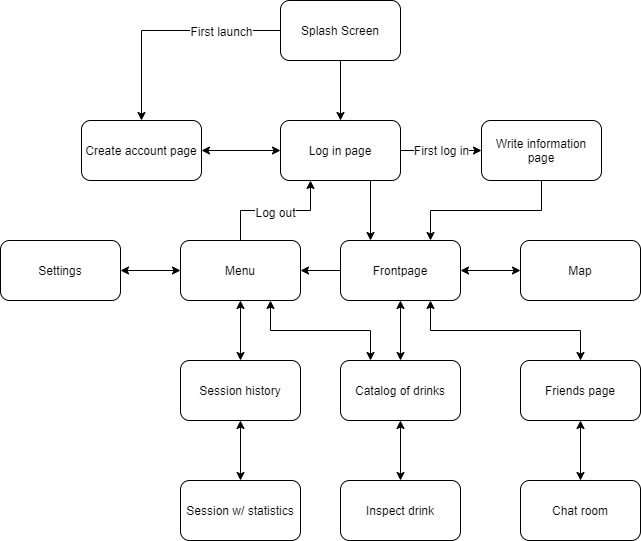
\includegraphics[scale=0.5]{images/lille_promille_float_diagram.drawio.png}
    \caption{Skisse som viser hvor man kan navigere seg til fra hvilke sider i appen.}
\end{figure}

\subsubsection{Navigation Pattern}
Bla bla bla

\subsection{Teknisk oppbygging}
Blablabla

\subsubsection{Lagring og uthenting av data}
Blablabla

\subsubsection{Brukerhåndtering}
I am blue
Da ba de da ba die

\subsection{Ressurser}
\subsubsection{Services}

\subsubsection{Fragmenter}
Siden vi bruker Navigation Component biblioteket, er det best praksise å bytte ut sidene via fragmenter. Vi har derfor delt opp appen i tre aktiviteter, hvor vi bytter ut fragmenter i hver av aktivitetene. Dette er både for å gjøre koden mer lesbar ved å abstrahere i logiske inndelinger og for å skille på de forskjellige navigasjonsmetodene, siden bottom-navigation og navigation-drawer kun finnes i hovedaktiviteten.

\subsubsection{Bilder}
Bilder i appen vil bestå av ikoner, logoer, emojier og eventuelt profilbilder. Ikonene brukes til å veilede brukeren der det er raskere å oppfatte ikonet enn å det er å lese teksten, for eksempel til navigasjonspunktene i bottom-navigation og navigation-drawer. Ikonene er en blanding av lånte og egenskapte ikoner som følger design prinsippene til Material Design dokumentasjonen(1).

Lille promille logoen har vi designet og laget selv. Det vil også være flere versjoner av logoen til de forskjellige seksjonene i appen der det er passende. For eksempel i sprutskjermen viser den hele logoen, som inkluderer teksten, mens i appikonet bruker den en minimalisert versjon av logoen.

I vennesiden brukes emojier til å visualisere hvilken alkoholstatus vennene har. Vi tror dette er en smart løsning fordi mange brukere er allerede familiære med systemet som Snapchat bruker, hvor de forklarer forholdet man har til en venn. Til denne funksjonen bruker Lille promille standardemojiene til android.

Hvis ønskelig kan brukeren legge til sitt eget profilbilde i innstillingene. Dette profilbilde vises både i navigation-drawer ved brukernavnet og i vennesiden ved siden av navnet sitt. Bildet kan hentes fra kamerarullen eller kan tas direkte fra kameraet.

\subsubsection{Lyd}
Dette har vi ikke tenkt på hittil.

\subsubsection{Biblioteker}
Firebase/Firestore
Google ting til firestore
Navigation Component
JUnits til testing